% Created by tikzDevice version 0.12.3.2 on 2023-07-05 10:07:29
% !TEX encoding = UTF-8 Unicode
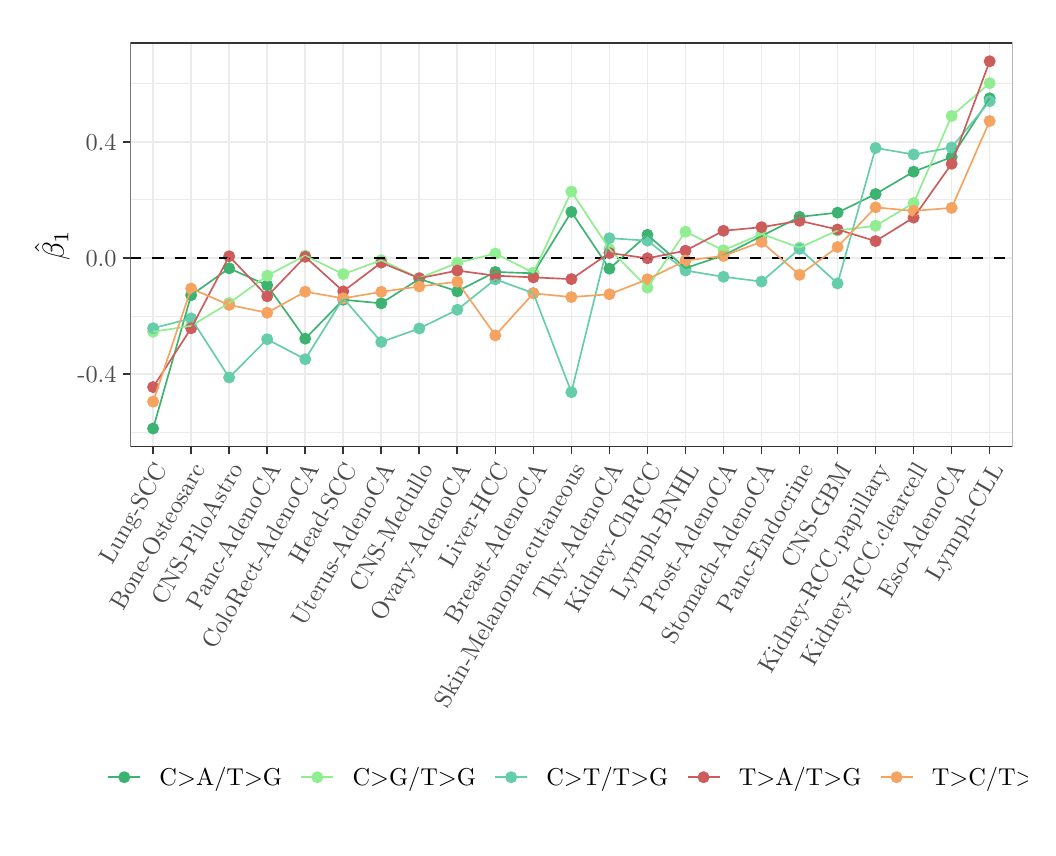
\begin{tikzpicture}[x=1pt,y=1pt]
\definecolor{fillColor}{RGB}{255,255,255}
\path[use as bounding box,fill=fillColor,fill opacity=0.00] (0,0) rectangle (361.35,289.08);
\begin{scope}
\path[clip] (  0.00,  0.00) rectangle (361.35,289.08);
\definecolor{drawColor}{RGB}{255,255,255}
\definecolor{fillColor}{RGB}{255,255,255}

\path[draw=drawColor,line width= 0.6pt,line join=round,line cap=round,fill=fillColor] (  0.00, -0.00) rectangle (361.35,289.08);
\end{scope}
\begin{scope}
\path[clip] ( 37.09,137.61) rectangle (355.85,283.58);
\definecolor{fillColor}{RGB}{255,255,255}

\path[fill=fillColor] ( 37.09,137.61) rectangle (355.85,283.58);
\definecolor{drawColor}{gray}{0.92}

\path[draw=drawColor,line width= 0.3pt,line join=round] ( 37.09,142.86) --
	(355.85,142.86);

\path[draw=drawColor,line width= 0.3pt,line join=round] ( 37.09,184.86) --
	(355.85,184.86);

\path[draw=drawColor,line width= 0.3pt,line join=round] ( 37.09,226.86) --
	(355.85,226.86);

\path[draw=drawColor,line width= 0.3pt,line join=round] ( 37.09,268.85) --
	(355.85,268.85);

\path[draw=drawColor,line width= 0.6pt,line join=round] ( 37.09,163.86) --
	(355.85,163.86);

\path[draw=drawColor,line width= 0.6pt,line join=round] ( 37.09,205.86) --
	(355.85,205.86);

\path[draw=drawColor,line width= 0.6pt,line join=round] ( 37.09,247.85) --
	(355.85,247.85);

\path[draw=drawColor,line width= 0.6pt,line join=round] ( 45.33,137.61) --
	( 45.33,283.58);

\path[draw=drawColor,line width= 0.6pt,line join=round] ( 59.07,137.61) --
	( 59.07,283.58);

\path[draw=drawColor,line width= 0.6pt,line join=round] ( 72.81,137.61) --
	( 72.81,283.58);

\path[draw=drawColor,line width= 0.6pt,line join=round] ( 86.55,137.61) --
	( 86.55,283.58);

\path[draw=drawColor,line width= 0.6pt,line join=round] (100.29,137.61) --
	(100.29,283.58);

\path[draw=drawColor,line width= 0.6pt,line join=round] (114.03,137.61) --
	(114.03,283.58);

\path[draw=drawColor,line width= 0.6pt,line join=round] (127.77,137.61) --
	(127.77,283.58);

\path[draw=drawColor,line width= 0.6pt,line join=round] (141.51,137.61) --
	(141.51,283.58);

\path[draw=drawColor,line width= 0.6pt,line join=round] (155.25,137.61) --
	(155.25,283.58);

\path[draw=drawColor,line width= 0.6pt,line join=round] (168.99,137.61) --
	(168.99,283.58);

\path[draw=drawColor,line width= 0.6pt,line join=round] (182.73,137.61) --
	(182.73,283.58);

\path[draw=drawColor,line width= 0.6pt,line join=round] (196.47,137.61) --
	(196.47,283.58);

\path[draw=drawColor,line width= 0.6pt,line join=round] (210.21,137.61) --
	(210.21,283.58);

\path[draw=drawColor,line width= 0.6pt,line join=round] (223.95,137.61) --
	(223.95,283.58);

\path[draw=drawColor,line width= 0.6pt,line join=round] (237.69,137.61) --
	(237.69,283.58);

\path[draw=drawColor,line width= 0.6pt,line join=round] (251.43,137.61) --
	(251.43,283.58);

\path[draw=drawColor,line width= 0.6pt,line join=round] (265.17,137.61) --
	(265.17,283.58);

\path[draw=drawColor,line width= 0.6pt,line join=round] (278.91,137.61) --
	(278.91,283.58);

\path[draw=drawColor,line width= 0.6pt,line join=round] (292.65,137.61) --
	(292.65,283.58);

\path[draw=drawColor,line width= 0.6pt,line join=round] (306.39,137.61) --
	(306.39,283.58);

\path[draw=drawColor,line width= 0.6pt,line join=round] (320.13,137.61) --
	(320.13,283.58);

\path[draw=drawColor,line width= 0.6pt,line join=round] (333.87,137.61) --
	(333.87,283.58);

\path[draw=drawColor,line width= 0.6pt,line join=round] (347.61,137.61) --
	(347.61,283.58);
\definecolor{drawColor}{RGB}{60,179,113}
\definecolor{fillColor}{RGB}{60,179,113}

\path[draw=drawColor,line width= 0.4pt,line join=round,line cap=round,fill=fillColor] ( 59.07,192.41) circle (  1.96);
\definecolor{drawColor}{RGB}{144,238,144}
\definecolor{fillColor}{RGB}{144,238,144}

\path[draw=drawColor,line width= 0.4pt,line join=round,line cap=round,fill=fillColor] ( 59.07,181.32) circle (  1.96);
\definecolor{drawColor}{RGB}{102,205,170}
\definecolor{fillColor}{RGB}{102,205,170}

\path[draw=drawColor,line width= 0.4pt,line join=round,line cap=round,fill=fillColor] ( 59.07,184.02) circle (  1.96);
\definecolor{drawColor}{RGB}{205,92,92}
\definecolor{fillColor}{RGB}{205,92,92}

\path[draw=drawColor,line width= 0.4pt,line join=round,line cap=round,fill=fillColor] ( 59.07,180.46) circle (  1.96);
\definecolor{drawColor}{RGB}{244,164,96}
\definecolor{fillColor}{RGB}{244,164,96}

\path[draw=drawColor,line width= 0.4pt,line join=round,line cap=round,fill=fillColor] ( 59.07,194.80) circle (  1.96);
\definecolor{drawColor}{RGB}{60,179,113}
\definecolor{fillColor}{RGB}{60,179,113}

\path[draw=drawColor,line width= 0.4pt,line join=round,line cap=round,fill=fillColor] (182.73,200.32) circle (  1.96);
\definecolor{drawColor}{RGB}{144,238,144}
\definecolor{fillColor}{RGB}{144,238,144}

\path[draw=drawColor,line width= 0.4pt,line join=round,line cap=round,fill=fillColor] (182.73,200.54) circle (  1.96);
\definecolor{drawColor}{RGB}{102,205,170}
\definecolor{fillColor}{RGB}{102,205,170}

\path[draw=drawColor,line width= 0.4pt,line join=round,line cap=round,fill=fillColor] (182.73,193.16) circle (  1.96);
\definecolor{drawColor}{RGB}{205,92,92}
\definecolor{fillColor}{RGB}{205,92,92}

\path[draw=drawColor,line width= 0.4pt,line join=round,line cap=round,fill=fillColor] (182.73,198.85) circle (  1.96);
\definecolor{drawColor}{RGB}{244,164,96}
\definecolor{fillColor}{RGB}{244,164,96}

\path[draw=drawColor,line width= 0.4pt,line join=round,line cap=round,fill=fillColor] (182.73,193.07) circle (  1.96);
\definecolor{drawColor}{RGB}{60,179,113}
\definecolor{fillColor}{RGB}{60,179,113}

\path[draw=drawColor,line width= 0.4pt,line join=round,line cap=round,fill=fillColor] (292.65,222.24) circle (  1.96);
\definecolor{drawColor}{RGB}{144,238,144}
\definecolor{fillColor}{RGB}{144,238,144}

\path[draw=drawColor,line width= 0.4pt,line join=round,line cap=round,fill=fillColor] (292.65,215.79) circle (  1.96);
\definecolor{drawColor}{RGB}{102,205,170}
\definecolor{fillColor}{RGB}{102,205,170}

\path[draw=drawColor,line width= 0.4pt,line join=round,line cap=round,fill=fillColor] (292.65,196.66) circle (  1.96);
\definecolor{drawColor}{RGB}{205,92,92}
\definecolor{fillColor}{RGB}{205,92,92}

\path[draw=drawColor,line width= 0.4pt,line join=round,line cap=round,fill=fillColor] (292.65,216.15) circle (  1.96);
\definecolor{drawColor}{RGB}{244,164,96}
\definecolor{fillColor}{RGB}{244,164,96}

\path[draw=drawColor,line width= 0.4pt,line join=round,line cap=round,fill=fillColor] (292.65,209.82) circle (  1.96);
\definecolor{drawColor}{RGB}{60,179,113}
\definecolor{fillColor}{RGB}{60,179,113}

\path[draw=drawColor,line width= 0.4pt,line join=round,line cap=round,fill=fillColor] (141.51,198.31) circle (  1.96);
\definecolor{drawColor}{RGB}{144,238,144}
\definecolor{fillColor}{RGB}{144,238,144}

\path[draw=drawColor,line width= 0.4pt,line join=round,line cap=round,fill=fillColor] (141.51,198.58) circle (  1.96);
\definecolor{drawColor}{RGB}{102,205,170}
\definecolor{fillColor}{RGB}{102,205,170}

\path[draw=drawColor,line width= 0.4pt,line join=round,line cap=round,fill=fillColor] (141.51,180.39) circle (  1.96);
\definecolor{drawColor}{RGB}{205,92,92}
\definecolor{fillColor}{RGB}{205,92,92}

\path[draw=drawColor,line width= 0.4pt,line join=round,line cap=round,fill=fillColor] (141.51,198.53) circle (  1.96);
\definecolor{drawColor}{RGB}{244,164,96}
\definecolor{fillColor}{RGB}{244,164,96}

\path[draw=drawColor,line width= 0.4pt,line join=round,line cap=round,fill=fillColor] (141.51,195.56) circle (  1.96);
\definecolor{drawColor}{RGB}{60,179,113}
\definecolor{fillColor}{RGB}{60,179,113}

\path[draw=drawColor,line width= 0.4pt,line join=round,line cap=round,fill=fillColor] ( 72.81,202.12) circle (  1.96);
\definecolor{drawColor}{RGB}{144,238,144}
\definecolor{fillColor}{RGB}{144,238,144}

\path[draw=drawColor,line width= 0.4pt,line join=round,line cap=round,fill=fillColor] ( 72.81,189.57) circle (  1.96);
\definecolor{drawColor}{RGB}{102,205,170}
\definecolor{fillColor}{RGB}{102,205,170}

\path[draw=drawColor,line width= 0.4pt,line join=round,line cap=round,fill=fillColor] ( 72.81,162.67) circle (  1.96);
\definecolor{drawColor}{RGB}{205,92,92}
\definecolor{fillColor}{RGB}{205,92,92}

\path[draw=drawColor,line width= 0.4pt,line join=round,line cap=round,fill=fillColor] ( 72.81,206.48) circle (  1.96);
\definecolor{drawColor}{RGB}{244,164,96}
\definecolor{fillColor}{RGB}{244,164,96}

\path[draw=drawColor,line width= 0.4pt,line join=round,line cap=round,fill=fillColor] ( 72.81,188.88) circle (  1.96);
\definecolor{drawColor}{RGB}{60,179,113}
\definecolor{fillColor}{RGB}{60,179,113}

\path[draw=drawColor,line width= 0.4pt,line join=round,line cap=round,fill=fillColor] (100.29,176.69) circle (  1.96);
\definecolor{drawColor}{RGB}{144,238,144}
\definecolor{fillColor}{RGB}{144,238,144}

\path[draw=drawColor,line width= 0.4pt,line join=round,line cap=round,fill=fillColor] (100.29,206.73) circle (  1.96);
\definecolor{drawColor}{RGB}{102,205,170}
\definecolor{fillColor}{RGB}{102,205,170}

\path[draw=drawColor,line width= 0.4pt,line join=round,line cap=round,fill=fillColor] (100.29,169.26) circle (  1.96);
\definecolor{drawColor}{RGB}{205,92,92}
\definecolor{fillColor}{RGB}{205,92,92}

\path[draw=drawColor,line width= 0.4pt,line join=round,line cap=round,fill=fillColor] (100.29,206.29) circle (  1.96);
\definecolor{drawColor}{RGB}{244,164,96}
\definecolor{fillColor}{RGB}{244,164,96}

\path[draw=drawColor,line width= 0.4pt,line join=round,line cap=round,fill=fillColor] (100.29,193.67) circle (  1.96);
\definecolor{drawColor}{RGB}{60,179,113}
\definecolor{fillColor}{RGB}{60,179,113}

\path[draw=drawColor,line width= 0.4pt,line join=round,line cap=round,fill=fillColor] (333.87,242.30) circle (  1.96);
\definecolor{drawColor}{RGB}{144,238,144}
\definecolor{fillColor}{RGB}{144,238,144}

\path[draw=drawColor,line width= 0.4pt,line join=round,line cap=round,fill=fillColor] (333.87,257.17) circle (  1.96);
\definecolor{drawColor}{RGB}{102,205,170}
\definecolor{fillColor}{RGB}{102,205,170}

\path[draw=drawColor,line width= 0.4pt,line join=round,line cap=round,fill=fillColor] (333.87,245.78) circle (  1.96);
\definecolor{drawColor}{RGB}{205,92,92}
\definecolor{fillColor}{RGB}{205,92,92}

\path[draw=drawColor,line width= 0.4pt,line join=round,line cap=round,fill=fillColor] (333.87,239.89) circle (  1.96);
\definecolor{drawColor}{RGB}{244,164,96}
\definecolor{fillColor}{RGB}{244,164,96}

\path[draw=drawColor,line width= 0.4pt,line join=round,line cap=round,fill=fillColor] (333.87,223.95) circle (  1.96);
\definecolor{drawColor}{RGB}{60,179,113}
\definecolor{fillColor}{RGB}{60,179,113}

\path[draw=drawColor,line width= 0.4pt,line join=round,line cap=round,fill=fillColor] (114.03,190.77) circle (  1.96);
\definecolor{drawColor}{RGB}{144,238,144}
\definecolor{fillColor}{RGB}{144,238,144}

\path[draw=drawColor,line width= 0.4pt,line join=round,line cap=round,fill=fillColor] (114.03,200.02) circle (  1.96);
\definecolor{drawColor}{RGB}{102,205,170}
\definecolor{fillColor}{RGB}{102,205,170}

\path[draw=drawColor,line width= 0.4pt,line join=round,line cap=round,fill=fillColor] (114.03,191.33) circle (  1.96);
\definecolor{drawColor}{RGB}{205,92,92}
\definecolor{fillColor}{RGB}{205,92,92}

\path[draw=drawColor,line width= 0.4pt,line join=round,line cap=round,fill=fillColor] (114.03,193.79) circle (  1.96);
\definecolor{drawColor}{RGB}{244,164,96}
\definecolor{fillColor}{RGB}{244,164,96}

\path[draw=drawColor,line width= 0.4pt,line join=round,line cap=round,fill=fillColor] (114.03,191.27) circle (  1.96);
\definecolor{drawColor}{RGB}{60,179,113}
\definecolor{fillColor}{RGB}{60,179,113}

\path[draw=drawColor,line width= 0.4pt,line join=round,line cap=round,fill=fillColor] (223.95,214.22) circle (  1.96);
\definecolor{drawColor}{RGB}{144,238,144}
\definecolor{fillColor}{RGB}{144,238,144}

\path[draw=drawColor,line width= 0.4pt,line join=round,line cap=round,fill=fillColor] (223.95,195.16) circle (  1.96);
\definecolor{drawColor}{RGB}{102,205,170}
\definecolor{fillColor}{RGB}{102,205,170}

\path[draw=drawColor,line width= 0.4pt,line join=round,line cap=round,fill=fillColor] (223.95,212.12) circle (  1.96);
\definecolor{drawColor}{RGB}{205,92,92}
\definecolor{fillColor}{RGB}{205,92,92}

\path[draw=drawColor,line width= 0.4pt,line join=round,line cap=round,fill=fillColor] (223.95,205.75) circle (  1.96);
\definecolor{drawColor}{RGB}{244,164,96}
\definecolor{fillColor}{RGB}{244,164,96}

\path[draw=drawColor,line width= 0.4pt,line join=round,line cap=round,fill=fillColor] (223.95,198.15) circle (  1.96);
\definecolor{drawColor}{RGB}{60,179,113}
\definecolor{fillColor}{RGB}{60,179,113}

\path[draw=drawColor,line width= 0.4pt,line join=round,line cap=round,fill=fillColor] (320.13,237.04) circle (  1.96);
\definecolor{drawColor}{RGB}{144,238,144}
\definecolor{fillColor}{RGB}{144,238,144}

\path[draw=drawColor,line width= 0.4pt,line join=round,line cap=round,fill=fillColor] (320.13,225.69) circle (  1.96);
\definecolor{drawColor}{RGB}{102,205,170}
\definecolor{fillColor}{RGB}{102,205,170}

\path[draw=drawColor,line width= 0.4pt,line join=round,line cap=round,fill=fillColor] (320.13,243.26) circle (  1.96);
\definecolor{drawColor}{RGB}{205,92,92}
\definecolor{fillColor}{RGB}{205,92,92}

\path[draw=drawColor,line width= 0.4pt,line join=round,line cap=round,fill=fillColor] (320.13,220.45) circle (  1.96);
\definecolor{drawColor}{RGB}{244,164,96}
\definecolor{fillColor}{RGB}{244,164,96}

\path[draw=drawColor,line width= 0.4pt,line join=round,line cap=round,fill=fillColor] (320.13,222.88) circle (  1.96);
\definecolor{drawColor}{RGB}{60,179,113}
\definecolor{fillColor}{RGB}{60,179,113}

\path[draw=drawColor,line width= 0.4pt,line join=round,line cap=round,fill=fillColor] (306.39,228.96) circle (  1.96);
\definecolor{drawColor}{RGB}{144,238,144}
\definecolor{fillColor}{RGB}{144,238,144}

\path[draw=drawColor,line width= 0.4pt,line join=round,line cap=round,fill=fillColor] (306.39,217.49) circle (  1.96);
\definecolor{drawColor}{RGB}{102,205,170}
\definecolor{fillColor}{RGB}{102,205,170}

\path[draw=drawColor,line width= 0.4pt,line join=round,line cap=round,fill=fillColor] (306.39,245.60) circle (  1.96);
\definecolor{drawColor}{RGB}{205,92,92}
\definecolor{fillColor}{RGB}{205,92,92}

\path[draw=drawColor,line width= 0.4pt,line join=round,line cap=round,fill=fillColor] (306.39,211.96) circle (  1.96);
\definecolor{drawColor}{RGB}{244,164,96}
\definecolor{fillColor}{RGB}{244,164,96}

\path[draw=drawColor,line width= 0.4pt,line join=round,line cap=round,fill=fillColor] (306.39,224.14) circle (  1.96);
\definecolor{drawColor}{RGB}{60,179,113}
\definecolor{fillColor}{RGB}{60,179,113}

\path[draw=drawColor,line width= 0.4pt,line join=round,line cap=round,fill=fillColor] (168.99,200.81) circle (  1.96);
\definecolor{drawColor}{RGB}{144,238,144}
\definecolor{fillColor}{RGB}{144,238,144}

\path[draw=drawColor,line width= 0.4pt,line join=round,line cap=round,fill=fillColor] (168.99,207.46) circle (  1.96);
\definecolor{drawColor}{RGB}{102,205,170}
\definecolor{fillColor}{RGB}{102,205,170}

\path[draw=drawColor,line width= 0.4pt,line join=round,line cap=round,fill=fillColor] (168.99,198.14) circle (  1.96);
\definecolor{drawColor}{RGB}{205,92,92}
\definecolor{fillColor}{RGB}{205,92,92}

\path[draw=drawColor,line width= 0.4pt,line join=round,line cap=round,fill=fillColor] (168.99,199.46) circle (  1.96);
\definecolor{drawColor}{RGB}{244,164,96}
\definecolor{fillColor}{RGB}{244,164,96}

\path[draw=drawColor,line width= 0.4pt,line join=round,line cap=round,fill=fillColor] (168.99,177.89) circle (  1.96);
\definecolor{drawColor}{RGB}{60,179,113}
\definecolor{fillColor}{RGB}{60,179,113}

\path[draw=drawColor,line width= 0.4pt,line join=round,line cap=round,fill=fillColor] ( 45.33,144.24) circle (  1.96);
\definecolor{drawColor}{RGB}{144,238,144}
\definecolor{fillColor}{RGB}{144,238,144}

\path[draw=drawColor,line width= 0.4pt,line join=round,line cap=round,fill=fillColor] ( 45.33,179.20) circle (  1.96);
\definecolor{drawColor}{RGB}{102,205,170}
\definecolor{fillColor}{RGB}{102,205,170}

\path[draw=drawColor,line width= 0.4pt,line join=round,line cap=round,fill=fillColor] ( 45.33,180.48) circle (  1.96);
\definecolor{drawColor}{RGB}{205,92,92}
\definecolor{fillColor}{RGB}{205,92,92}

\path[draw=drawColor,line width= 0.4pt,line join=round,line cap=round,fill=fillColor] ( 45.33,159.20) circle (  1.96);
\definecolor{drawColor}{RGB}{244,164,96}
\definecolor{fillColor}{RGB}{244,164,96}

\path[draw=drawColor,line width= 0.4pt,line join=round,line cap=round,fill=fillColor] ( 45.33,153.97) circle (  1.96);
\definecolor{drawColor}{RGB}{60,179,113}
\definecolor{fillColor}{RGB}{60,179,113}

\path[draw=drawColor,line width= 0.4pt,line join=round,line cap=round,fill=fillColor] (237.69,202.18) circle (  1.96);
\definecolor{drawColor}{RGB}{144,238,144}
\definecolor{fillColor}{RGB}{144,238,144}

\path[draw=drawColor,line width= 0.4pt,line join=round,line cap=round,fill=fillColor] (237.69,215.35) circle (  1.96);
\definecolor{drawColor}{RGB}{102,205,170}
\definecolor{fillColor}{RGB}{102,205,170}

\path[draw=drawColor,line width= 0.4pt,line join=round,line cap=round,fill=fillColor] (237.69,201.32) circle (  1.96);
\definecolor{drawColor}{RGB}{205,92,92}
\definecolor{fillColor}{RGB}{205,92,92}

\path[draw=drawColor,line width= 0.4pt,line join=round,line cap=round,fill=fillColor] (237.69,208.49) circle (  1.96);
\definecolor{drawColor}{RGB}{244,164,96}
\definecolor{fillColor}{RGB}{244,164,96}

\path[draw=drawColor,line width= 0.4pt,line join=round,line cap=round,fill=fillColor] (237.69,204.93) circle (  1.96);
\definecolor{drawColor}{RGB}{60,179,113}
\definecolor{fillColor}{RGB}{60,179,113}

\path[draw=drawColor,line width= 0.4pt,line join=round,line cap=round,fill=fillColor] (347.61,263.55) circle (  1.96);
\definecolor{drawColor}{RGB}{144,238,144}
\definecolor{fillColor}{RGB}{144,238,144}

\path[draw=drawColor,line width= 0.4pt,line join=round,line cap=round,fill=fillColor] (347.61,269.03) circle (  1.96);
\definecolor{drawColor}{RGB}{102,205,170}
\definecolor{fillColor}{RGB}{102,205,170}

\path[draw=drawColor,line width= 0.4pt,line join=round,line cap=round,fill=fillColor] (347.61,262.52) circle (  1.96);
\definecolor{drawColor}{RGB}{205,92,92}
\definecolor{fillColor}{RGB}{205,92,92}

\path[draw=drawColor,line width= 0.4pt,line join=round,line cap=round,fill=fillColor] (347.61,276.94) circle (  1.96);
\definecolor{drawColor}{RGB}{244,164,96}
\definecolor{fillColor}{RGB}{244,164,96}

\path[draw=drawColor,line width= 0.4pt,line join=round,line cap=round,fill=fillColor] (347.61,255.33) circle (  1.96);
\definecolor{drawColor}{RGB}{60,179,113}
\definecolor{fillColor}{RGB}{60,179,113}

\path[draw=drawColor,line width= 0.4pt,line join=round,line cap=round,fill=fillColor] (155.25,193.81) circle (  1.96);
\definecolor{drawColor}{RGB}{144,238,144}
\definecolor{fillColor}{RGB}{144,238,144}

\path[draw=drawColor,line width= 0.4pt,line join=round,line cap=round,fill=fillColor] (155.25,204.08) circle (  1.96);
\definecolor{drawColor}{RGB}{102,205,170}
\definecolor{fillColor}{RGB}{102,205,170}

\path[draw=drawColor,line width= 0.4pt,line join=round,line cap=round,fill=fillColor] (155.25,187.16) circle (  1.96);
\definecolor{drawColor}{RGB}{205,92,92}
\definecolor{fillColor}{RGB}{205,92,92}

\path[draw=drawColor,line width= 0.4pt,line join=round,line cap=round,fill=fillColor] (155.25,201.30) circle (  1.96);
\definecolor{drawColor}{RGB}{244,164,96}
\definecolor{fillColor}{RGB}{244,164,96}

\path[draw=drawColor,line width= 0.4pt,line join=round,line cap=round,fill=fillColor] (155.25,197.27) circle (  1.96);
\definecolor{drawColor}{RGB}{60,179,113}
\definecolor{fillColor}{RGB}{60,179,113}

\path[draw=drawColor,line width= 0.4pt,line join=round,line cap=round,fill=fillColor] ( 86.55,195.98) circle (  1.96);
\definecolor{drawColor}{RGB}{144,238,144}
\definecolor{fillColor}{RGB}{144,238,144}

\path[draw=drawColor,line width= 0.4pt,line join=round,line cap=round,fill=fillColor] ( 86.55,199.45) circle (  1.96);
\definecolor{drawColor}{RGB}{102,205,170}
\definecolor{fillColor}{RGB}{102,205,170}

\path[draw=drawColor,line width= 0.4pt,line join=round,line cap=round,fill=fillColor] ( 86.55,176.49) circle (  1.96);
\definecolor{drawColor}{RGB}{205,92,92}
\definecolor{fillColor}{RGB}{205,92,92}

\path[draw=drawColor,line width= 0.4pt,line join=round,line cap=round,fill=fillColor] ( 86.55,192.01) circle (  1.96);
\definecolor{drawColor}{RGB}{244,164,96}
\definecolor{fillColor}{RGB}{244,164,96}

\path[draw=drawColor,line width= 0.4pt,line join=round,line cap=round,fill=fillColor] ( 86.55,186.08) circle (  1.96);
\definecolor{drawColor}{RGB}{60,179,113}
\definecolor{fillColor}{RGB}{60,179,113}

\path[draw=drawColor,line width= 0.4pt,line join=round,line cap=round,fill=fillColor] (278.91,220.71) circle (  1.96);
\definecolor{drawColor}{RGB}{144,238,144}
\definecolor{fillColor}{RGB}{144,238,144}

\path[draw=drawColor,line width= 0.4pt,line join=round,line cap=round,fill=fillColor] (278.91,209.58) circle (  1.96);
\definecolor{drawColor}{RGB}{102,205,170}
\definecolor{fillColor}{RGB}{102,205,170}

\path[draw=drawColor,line width= 0.4pt,line join=round,line cap=round,fill=fillColor] (278.91,209.16) circle (  1.96);
\definecolor{drawColor}{RGB}{205,92,92}
\definecolor{fillColor}{RGB}{205,92,92}

\path[draw=drawColor,line width= 0.4pt,line join=round,line cap=round,fill=fillColor] (278.91,219.30) circle (  1.96);
\definecolor{drawColor}{RGB}{244,164,96}
\definecolor{fillColor}{RGB}{244,164,96}

\path[draw=drawColor,line width= 0.4pt,line join=round,line cap=round,fill=fillColor] (278.91,199.76) circle (  1.96);
\definecolor{drawColor}{RGB}{60,179,113}
\definecolor{fillColor}{RGB}{60,179,113}

\path[draw=drawColor,line width= 0.4pt,line join=round,line cap=round,fill=fillColor] (251.43,206.78) circle (  1.96);
\definecolor{drawColor}{RGB}{144,238,144}
\definecolor{fillColor}{RGB}{144,238,144}

\path[draw=drawColor,line width= 0.4pt,line join=round,line cap=round,fill=fillColor] (251.43,208.64) circle (  1.96);
\definecolor{drawColor}{RGB}{102,205,170}
\definecolor{fillColor}{RGB}{102,205,170}

\path[draw=drawColor,line width= 0.4pt,line join=round,line cap=round,fill=fillColor] (251.43,199.05) circle (  1.96);
\definecolor{drawColor}{RGB}{205,92,92}
\definecolor{fillColor}{RGB}{205,92,92}

\path[draw=drawColor,line width= 0.4pt,line join=round,line cap=round,fill=fillColor] (251.43,215.69) circle (  1.96);
\definecolor{drawColor}{RGB}{244,164,96}
\definecolor{fillColor}{RGB}{244,164,96}

\path[draw=drawColor,line width= 0.4pt,line join=round,line cap=round,fill=fillColor] (251.43,206.60) circle (  1.96);
\definecolor{drawColor}{RGB}{60,179,113}
\definecolor{fillColor}{RGB}{60,179,113}

\path[draw=drawColor,line width= 0.4pt,line join=round,line cap=round,fill=fillColor] (196.47,222.50) circle (  1.96);
\definecolor{drawColor}{RGB}{144,238,144}
\definecolor{fillColor}{RGB}{144,238,144}

\path[draw=drawColor,line width= 0.4pt,line join=round,line cap=round,fill=fillColor] (196.47,229.87) circle (  1.96);
\definecolor{drawColor}{RGB}{102,205,170}
\definecolor{fillColor}{RGB}{102,205,170}

\path[draw=drawColor,line width= 0.4pt,line join=round,line cap=round,fill=fillColor] (196.47,157.36) circle (  1.96);
\definecolor{drawColor}{RGB}{205,92,92}
\definecolor{fillColor}{RGB}{205,92,92}

\path[draw=drawColor,line width= 0.4pt,line join=round,line cap=round,fill=fillColor] (196.47,198.22) circle (  1.96);
\definecolor{drawColor}{RGB}{244,164,96}
\definecolor{fillColor}{RGB}{244,164,96}

\path[draw=drawColor,line width= 0.4pt,line join=round,line cap=round,fill=fillColor] (196.47,191.73) circle (  1.96);
\definecolor{drawColor}{RGB}{60,179,113}
\definecolor{fillColor}{RGB}{60,179,113}

\path[draw=drawColor,line width= 0.4pt,line join=round,line cap=round,fill=fillColor] (265.17,213.77) circle (  1.96);
\definecolor{drawColor}{RGB}{144,238,144}
\definecolor{fillColor}{RGB}{144,238,144}

\path[draw=drawColor,line width= 0.4pt,line join=round,line cap=round,fill=fillColor] (265.17,214.52) circle (  1.96);
\definecolor{drawColor}{RGB}{102,205,170}
\definecolor{fillColor}{RGB}{102,205,170}

\path[draw=drawColor,line width= 0.4pt,line join=round,line cap=round,fill=fillColor] (265.17,197.35) circle (  1.96);
\definecolor{drawColor}{RGB}{205,92,92}
\definecolor{fillColor}{RGB}{205,92,92}

\path[draw=drawColor,line width= 0.4pt,line join=round,line cap=round,fill=fillColor] (265.17,216.98) circle (  1.96);
\definecolor{drawColor}{RGB}{244,164,96}
\definecolor{fillColor}{RGB}{244,164,96}

\path[draw=drawColor,line width= 0.4pt,line join=round,line cap=round,fill=fillColor] (265.17,211.67) circle (  1.96);
\definecolor{drawColor}{RGB}{60,179,113}
\definecolor{fillColor}{RGB}{60,179,113}

\path[draw=drawColor,line width= 0.4pt,line join=round,line cap=round,fill=fillColor] (210.21,201.98) circle (  1.96);
\definecolor{drawColor}{RGB}{144,238,144}
\definecolor{fillColor}{RGB}{144,238,144}

\path[draw=drawColor,line width= 0.4pt,line join=round,line cap=round,fill=fillColor] (210.21,209.11) circle (  1.96);
\definecolor{drawColor}{RGB}{102,205,170}
\definecolor{fillColor}{RGB}{102,205,170}

\path[draw=drawColor,line width= 0.4pt,line join=round,line cap=round,fill=fillColor] (210.21,213.00) circle (  1.96);
\definecolor{drawColor}{RGB}{205,92,92}
\definecolor{fillColor}{RGB}{205,92,92}

\path[draw=drawColor,line width= 0.4pt,line join=round,line cap=round,fill=fillColor] (210.21,207.66) circle (  1.96);
\definecolor{drawColor}{RGB}{244,164,96}
\definecolor{fillColor}{RGB}{244,164,96}

\path[draw=drawColor,line width= 0.4pt,line join=round,line cap=round,fill=fillColor] (210.21,192.74) circle (  1.96);
\definecolor{drawColor}{RGB}{60,179,113}
\definecolor{fillColor}{RGB}{60,179,113}

\path[draw=drawColor,line width= 0.4pt,line join=round,line cap=round,fill=fillColor] (127.77,189.47) circle (  1.96);
\definecolor{drawColor}{RGB}{144,238,144}
\definecolor{fillColor}{RGB}{144,238,144}

\path[draw=drawColor,line width= 0.4pt,line join=round,line cap=round,fill=fillColor] (127.77,205.04) circle (  1.96);
\definecolor{drawColor}{RGB}{102,205,170}
\definecolor{fillColor}{RGB}{102,205,170}

\path[draw=drawColor,line width= 0.4pt,line join=round,line cap=round,fill=fillColor] (127.77,175.50) circle (  1.96);
\definecolor{drawColor}{RGB}{205,92,92}
\definecolor{fillColor}{RGB}{205,92,92}

\path[draw=drawColor,line width= 0.4pt,line join=round,line cap=round,fill=fillColor] (127.77,204.19) circle (  1.96);
\definecolor{drawColor}{RGB}{244,164,96}
\definecolor{fillColor}{RGB}{244,164,96}

\path[draw=drawColor,line width= 0.4pt,line join=round,line cap=round,fill=fillColor] (127.77,193.63) circle (  1.96);
\definecolor{drawColor}{RGB}{0,0,0}

\path[draw=drawColor,line width= 0.6pt,dash pattern=on 4pt off 4pt ,line join=round] ( 37.09,205.86) -- (355.85,205.86);
\definecolor{drawColor}{RGB}{60,179,113}

\path[draw=drawColor,line width= 0.6pt,line join=round] ( 45.33,144.24) --
	( 59.07,192.41) --
	( 72.81,202.12) --
	( 86.55,195.98) --
	(100.29,176.69) --
	(114.03,190.77) --
	(127.77,189.47) --
	(141.51,198.31) --
	(155.25,193.81) --
	(168.99,200.81) --
	(182.73,200.32) --
	(196.47,222.50) --
	(210.21,201.98) --
	(223.95,214.22) --
	(237.69,202.18) --
	(251.43,206.78) --
	(265.17,213.77) --
	(278.91,220.71) --
	(292.65,222.24) --
	(306.39,228.96) --
	(320.13,237.04) --
	(333.87,242.30) --
	(347.61,263.55);
\definecolor{drawColor}{RGB}{144,238,144}

\path[draw=drawColor,line width= 0.6pt,line join=round] ( 45.33,179.20) --
	( 59.07,181.32) --
	( 72.81,189.57) --
	( 86.55,199.45) --
	(100.29,206.73) --
	(114.03,200.02) --
	(127.77,205.04) --
	(141.51,198.58) --
	(155.25,204.08) --
	(168.99,207.46) --
	(182.73,200.54) --
	(196.47,229.87) --
	(210.21,209.11) --
	(223.95,195.16) --
	(237.69,215.35) --
	(251.43,208.64) --
	(265.17,214.52) --
	(278.91,209.58) --
	(292.65,215.79) --
	(306.39,217.49) --
	(320.13,225.69) --
	(333.87,257.17) --
	(347.61,269.03);
\definecolor{drawColor}{RGB}{102,205,170}

\path[draw=drawColor,line width= 0.6pt,line join=round] ( 45.33,180.48) --
	( 59.07,184.02) --
	( 72.81,162.67) --
	( 86.55,176.49) --
	(100.29,169.26) --
	(114.03,191.33) --
	(127.77,175.50) --
	(141.51,180.39) --
	(155.25,187.16) --
	(168.99,198.14) --
	(182.73,193.16) --
	(196.47,157.36) --
	(210.21,213.00) --
	(223.95,212.12) --
	(237.69,201.32) --
	(251.43,199.05) --
	(265.17,197.35) --
	(278.91,209.16) --
	(292.65,196.66) --
	(306.39,245.60) --
	(320.13,243.26) --
	(333.87,245.78) --
	(347.61,262.52);
\definecolor{drawColor}{RGB}{205,92,92}

\path[draw=drawColor,line width= 0.6pt,line join=round] ( 45.33,159.20) --
	( 59.07,180.46) --
	( 72.81,206.48) --
	( 86.55,192.01) --
	(100.29,206.29) --
	(114.03,193.79) --
	(127.77,204.19) --
	(141.51,198.53) --
	(155.25,201.30) --
	(168.99,199.46) --
	(182.73,198.85) --
	(196.47,198.22) --
	(210.21,207.66) --
	(223.95,205.75) --
	(237.69,208.49) --
	(251.43,215.69) --
	(265.17,216.98) --
	(278.91,219.30) --
	(292.65,216.15) --
	(306.39,211.96) --
	(320.13,220.45) --
	(333.87,239.89) --
	(347.61,276.94);
\definecolor{drawColor}{RGB}{244,164,96}

\path[draw=drawColor,line width= 0.6pt,line join=round] ( 45.33,153.97) --
	( 59.07,194.80) --
	( 72.81,188.88) --
	( 86.55,186.08) --
	(100.29,193.67) --
	(114.03,191.27) --
	(127.77,193.63) --
	(141.51,195.56) --
	(155.25,197.27) --
	(168.99,177.89) --
	(182.73,193.07) --
	(196.47,191.73) --
	(210.21,192.74) --
	(223.95,198.15) --
	(237.69,204.93) --
	(251.43,206.60) --
	(265.17,211.67) --
	(278.91,199.76) --
	(292.65,209.82) --
	(306.39,224.14) --
	(320.13,222.88) --
	(333.87,223.95) --
	(347.61,255.33);
\definecolor{drawColor}{gray}{0.20}

\path[draw=drawColor,line width= 0.6pt,line join=round,line cap=round] ( 37.09,137.61) rectangle (355.85,283.58);
\end{scope}
\begin{scope}
\path[clip] (  0.00,  0.00) rectangle (361.35,289.08);
\definecolor{drawColor}{gray}{0.30}

\node[text=drawColor,anchor=base east,inner sep=0pt, outer sep=0pt, scale=  0.88] at ( 32.14,160.83) {-0.4};

\node[text=drawColor,anchor=base east,inner sep=0pt, outer sep=0pt, scale=  0.88] at ( 32.14,202.83) {0.0};

\node[text=drawColor,anchor=base east,inner sep=0pt, outer sep=0pt, scale=  0.88] at ( 32.14,244.82) {0.4};
\end{scope}
\begin{scope}
\path[clip] (  0.00,  0.00) rectangle (361.35,289.08);
\definecolor{drawColor}{gray}{0.20}

\path[draw=drawColor,line width= 0.6pt,line join=round] ( 34.34,163.86) --
	( 37.09,163.86);

\path[draw=drawColor,line width= 0.6pt,line join=round] ( 34.34,205.86) --
	( 37.09,205.86);

\path[draw=drawColor,line width= 0.6pt,line join=round] ( 34.34,247.85) --
	( 37.09,247.85);
\end{scope}
\begin{scope}
\path[clip] (  0.00,  0.00) rectangle (361.35,289.08);
\definecolor{drawColor}{gray}{0.20}

\path[draw=drawColor,line width= 0.6pt,line join=round] ( 45.33,134.86) --
	( 45.33,137.61);

\path[draw=drawColor,line width= 0.6pt,line join=round] ( 59.07,134.86) --
	( 59.07,137.61);

\path[draw=drawColor,line width= 0.6pt,line join=round] ( 72.81,134.86) --
	( 72.81,137.61);

\path[draw=drawColor,line width= 0.6pt,line join=round] ( 86.55,134.86) --
	( 86.55,137.61);

\path[draw=drawColor,line width= 0.6pt,line join=round] (100.29,134.86) --
	(100.29,137.61);

\path[draw=drawColor,line width= 0.6pt,line join=round] (114.03,134.86) --
	(114.03,137.61);

\path[draw=drawColor,line width= 0.6pt,line join=round] (127.77,134.86) --
	(127.77,137.61);

\path[draw=drawColor,line width= 0.6pt,line join=round] (141.51,134.86) --
	(141.51,137.61);

\path[draw=drawColor,line width= 0.6pt,line join=round] (155.25,134.86) --
	(155.25,137.61);

\path[draw=drawColor,line width= 0.6pt,line join=round] (168.99,134.86) --
	(168.99,137.61);

\path[draw=drawColor,line width= 0.6pt,line join=round] (182.73,134.86) --
	(182.73,137.61);

\path[draw=drawColor,line width= 0.6pt,line join=round] (196.47,134.86) --
	(196.47,137.61);

\path[draw=drawColor,line width= 0.6pt,line join=round] (210.21,134.86) --
	(210.21,137.61);

\path[draw=drawColor,line width= 0.6pt,line join=round] (223.95,134.86) --
	(223.95,137.61);

\path[draw=drawColor,line width= 0.6pt,line join=round] (237.69,134.86) --
	(237.69,137.61);

\path[draw=drawColor,line width= 0.6pt,line join=round] (251.43,134.86) --
	(251.43,137.61);

\path[draw=drawColor,line width= 0.6pt,line join=round] (265.17,134.86) --
	(265.17,137.61);

\path[draw=drawColor,line width= 0.6pt,line join=round] (278.91,134.86) --
	(278.91,137.61);

\path[draw=drawColor,line width= 0.6pt,line join=round] (292.65,134.86) --
	(292.65,137.61);

\path[draw=drawColor,line width= 0.6pt,line join=round] (306.39,134.86) --
	(306.39,137.61);

\path[draw=drawColor,line width= 0.6pt,line join=round] (320.13,134.86) --
	(320.13,137.61);

\path[draw=drawColor,line width= 0.6pt,line join=round] (333.87,134.86) --
	(333.87,137.61);

\path[draw=drawColor,line width= 0.6pt,line join=round] (347.61,134.86) --
	(347.61,137.61);
\end{scope}
\begin{scope}
\path[clip] (  0.00,  0.00) rectangle (361.35,289.08);
\definecolor{drawColor}{gray}{0.30}

\node[text=drawColor,rotate= 60.00,anchor=base east,inner sep=0pt, outer sep=0pt, scale=  0.88] at ( 50.58,129.63) {Lung-SCC};

\node[text=drawColor,rotate= 60.00,anchor=base east,inner sep=0pt, outer sep=0pt, scale=  0.88] at ( 64.32,129.63) {Bone-Osteosarc};

\node[text=drawColor,rotate= 60.00,anchor=base east,inner sep=0pt, outer sep=0pt, scale=  0.88] at ( 78.06,129.63) {CNS-PiloAstro};

\node[text=drawColor,rotate= 60.00,anchor=base east,inner sep=0pt, outer sep=0pt, scale=  0.88] at ( 91.80,129.63) {Panc-AdenoCA};

\node[text=drawColor,rotate= 60.00,anchor=base east,inner sep=0pt, outer sep=0pt, scale=  0.88] at (105.54,129.63) {ColoRect-AdenoCA};

\node[text=drawColor,rotate= 60.00,anchor=base east,inner sep=0pt, outer sep=0pt, scale=  0.88] at (119.28,129.63) {Head-SCC};

\node[text=drawColor,rotate= 60.00,anchor=base east,inner sep=0pt, outer sep=0pt, scale=  0.88] at (133.02,129.63) {Uterus-AdenoCA};

\node[text=drawColor,rotate= 60.00,anchor=base east,inner sep=0pt, outer sep=0pt, scale=  0.88] at (146.76,129.63) {CNS-Medullo};

\node[text=drawColor,rotate= 60.00,anchor=base east,inner sep=0pt, outer sep=0pt, scale=  0.88] at (160.50,129.63) {Ovary-AdenoCA};

\node[text=drawColor,rotate= 60.00,anchor=base east,inner sep=0pt, outer sep=0pt, scale=  0.88] at (174.24,129.63) {Liver-HCC};

\node[text=drawColor,rotate= 60.00,anchor=base east,inner sep=0pt, outer sep=0pt, scale=  0.88] at (187.98,129.63) {Breast-AdenoCA};

\node[text=drawColor,rotate= 60.00,anchor=base east,inner sep=0pt, outer sep=0pt, scale=  0.88] at (201.72,129.63) {Skin-Melanoma.cutaneous};

\node[text=drawColor,rotate= 60.00,anchor=base east,inner sep=0pt, outer sep=0pt, scale=  0.88] at (215.46,129.63) {Thy-AdenoCA};

\node[text=drawColor,rotate= 60.00,anchor=base east,inner sep=0pt, outer sep=0pt, scale=  0.88] at (229.20,129.63) {Kidney-ChRCC};

\node[text=drawColor,rotate= 60.00,anchor=base east,inner sep=0pt, outer sep=0pt, scale=  0.88] at (242.94,129.63) {Lymph-BNHL};

\node[text=drawColor,rotate= 60.00,anchor=base east,inner sep=0pt, outer sep=0pt, scale=  0.88] at (256.68,129.63) {Prost-AdenoCA};

\node[text=drawColor,rotate= 60.00,anchor=base east,inner sep=0pt, outer sep=0pt, scale=  0.88] at (270.42,129.63) {Stomach-AdenoCA};

\node[text=drawColor,rotate= 60.00,anchor=base east,inner sep=0pt, outer sep=0pt, scale=  0.88] at (284.16,129.63) {Panc-Endocrine};

\node[text=drawColor,rotate= 60.00,anchor=base east,inner sep=0pt, outer sep=0pt, scale=  0.88] at (297.90,129.63) {CNS-GBM};

\node[text=drawColor,rotate= 60.00,anchor=base east,inner sep=0pt, outer sep=0pt, scale=  0.88] at (311.64,129.63) {Kidney-RCC.papillary};

\node[text=drawColor,rotate= 60.00,anchor=base east,inner sep=0pt, outer sep=0pt, scale=  0.88] at (325.38,129.63) {Kidney-RCC.clearcell};

\node[text=drawColor,rotate= 60.00,anchor=base east,inner sep=0pt, outer sep=0pt, scale=  0.88] at (339.12,129.63) {Eso-AdenoCA};

\node[text=drawColor,rotate= 60.00,anchor=base east,inner sep=0pt, outer sep=0pt, scale=  0.88] at (352.85,129.63) {Lymph-CLL};
\end{scope}
\begin{scope}
\path[clip] (  0.00,  0.00) rectangle (361.35,289.08);
\definecolor{drawColor}{RGB}{0,0,0}

\node[text=drawColor,rotate= 90.00,anchor=base,inner sep=0pt, outer sep=0pt, scale=  1.10] at ( 13.08,210.59) {$\hat{\beta}_1$};
\end{scope}
\begin{scope}
\path[clip] (  0.00,  0.00) rectangle (361.35,289.08);
\definecolor{fillColor}{RGB}{255,255,255}

\path[fill=fillColor] ( 16.68,  5.50) rectangle (376.26, 30.95);
\end{scope}
\begin{scope}
\path[clip] (  0.00,  0.00) rectangle (361.35,289.08);
\definecolor{fillColor}{RGB}{255,255,255}

\path[fill=fillColor] ( 27.68, 11.00) rectangle ( 42.13, 25.45);
\end{scope}
\begin{scope}
\path[clip] (  0.00,  0.00) rectangle (361.35,289.08);
\definecolor{drawColor}{RGB}{60,179,113}
\definecolor{fillColor}{RGB}{60,179,113}

\path[draw=drawColor,line width= 0.4pt,line join=round,line cap=round,fill=fillColor] ( 34.91, 18.23) circle (  1.96);
\end{scope}
\begin{scope}
\path[clip] (  0.00,  0.00) rectangle (361.35,289.08);
\definecolor{drawColor}{RGB}{60,179,113}

\path[draw=drawColor,line width= 0.6pt,line join=round] ( 29.13, 18.23) -- ( 40.69, 18.23);
\end{scope}
\begin{scope}
\path[clip] (  0.00,  0.00) rectangle (361.35,289.08);
\definecolor{fillColor}{RGB}{255,255,255}

\path[fill=fillColor] ( 97.43, 11.00) rectangle (111.89, 25.45);
\end{scope}
\begin{scope}
\path[clip] (  0.00,  0.00) rectangle (361.35,289.08);
\definecolor{drawColor}{RGB}{144,238,144}
\definecolor{fillColor}{RGB}{144,238,144}

\path[draw=drawColor,line width= 0.4pt,line join=round,line cap=round,fill=fillColor] (104.66, 18.23) circle (  1.96);
\end{scope}
\begin{scope}
\path[clip] (  0.00,  0.00) rectangle (361.35,289.08);
\definecolor{drawColor}{RGB}{144,238,144}

\path[draw=drawColor,line width= 0.6pt,line join=round] ( 98.88, 18.23) -- (110.44, 18.23);
\end{scope}
\begin{scope}
\path[clip] (  0.00,  0.00) rectangle (361.35,289.08);
\definecolor{fillColor}{RGB}{255,255,255}

\path[fill=fillColor] (167.49, 11.00) rectangle (181.94, 25.45);
\end{scope}
\begin{scope}
\path[clip] (  0.00,  0.00) rectangle (361.35,289.08);
\definecolor{drawColor}{RGB}{102,205,170}
\definecolor{fillColor}{RGB}{102,205,170}

\path[draw=drawColor,line width= 0.4pt,line join=round,line cap=round,fill=fillColor] (174.72, 18.23) circle (  1.96);
\end{scope}
\begin{scope}
\path[clip] (  0.00,  0.00) rectangle (361.35,289.08);
\definecolor{drawColor}{RGB}{102,205,170}

\path[draw=drawColor,line width= 0.6pt,line join=round] (168.94, 18.23) -- (180.50, 18.23);
\end{scope}
\begin{scope}
\path[clip] (  0.00,  0.00) rectangle (361.35,289.08);
\definecolor{fillColor}{RGB}{255,255,255}

\path[fill=fillColor] (237.00, 11.00) rectangle (251.45, 25.45);
\end{scope}
\begin{scope}
\path[clip] (  0.00,  0.00) rectangle (361.35,289.08);
\definecolor{drawColor}{RGB}{205,92,92}
\definecolor{fillColor}{RGB}{205,92,92}

\path[draw=drawColor,line width= 0.4pt,line join=round,line cap=round,fill=fillColor] (244.23, 18.23) circle (  1.96);
\end{scope}
\begin{scope}
\path[clip] (  0.00,  0.00) rectangle (361.35,289.08);
\definecolor{drawColor}{RGB}{205,92,92}

\path[draw=drawColor,line width= 0.6pt,line join=round] (238.44, 18.23) -- (250.01, 18.23);
\end{scope}
\begin{scope}
\path[clip] (  0.00,  0.00) rectangle (361.35,289.08);
\definecolor{fillColor}{RGB}{255,255,255}

\path[fill=fillColor] (306.75, 11.00) rectangle (321.20, 25.45);
\end{scope}
\begin{scope}
\path[clip] (  0.00,  0.00) rectangle (361.35,289.08);
\definecolor{drawColor}{RGB}{244,164,96}
\definecolor{fillColor}{RGB}{244,164,96}

\path[draw=drawColor,line width= 0.4pt,line join=round,line cap=round,fill=fillColor] (313.98, 18.23) circle (  1.96);
\end{scope}
\begin{scope}
\path[clip] (  0.00,  0.00) rectangle (361.35,289.08);
\definecolor{drawColor}{RGB}{244,164,96}

\path[draw=drawColor,line width= 0.6pt,line join=round] (308.20, 18.23) -- (319.76, 18.23);
\end{scope}
\begin{scope}
\path[clip] (  0.00,  0.00) rectangle (361.35,289.08);
\definecolor{drawColor}{RGB}{0,0,0}

\node[text=drawColor,anchor=base west,inner sep=0pt, outer sep=0pt, scale=  0.88] at ( 47.63, 15.20) {C$>$A/T$>$G};
\end{scope}
\begin{scope}
\path[clip] (  0.00,  0.00) rectangle (361.35,289.08);
\definecolor{drawColor}{RGB}{0,0,0}

\node[text=drawColor,anchor=base west,inner sep=0pt, outer sep=0pt, scale=  0.88] at (117.39, 15.20) {C$>$G/T$>$G};
\end{scope}
\begin{scope}
\path[clip] (  0.00,  0.00) rectangle (361.35,289.08);
\definecolor{drawColor}{RGB}{0,0,0}

\node[text=drawColor,anchor=base west,inner sep=0pt, outer sep=0pt, scale=  0.88] at (187.44, 15.20) {C$>$T/T$>$G};
\end{scope}
\begin{scope}
\path[clip] (  0.00,  0.00) rectangle (361.35,289.08);
\definecolor{drawColor}{RGB}{0,0,0}

\node[text=drawColor,anchor=base west,inner sep=0pt, outer sep=0pt, scale=  0.88] at (256.95, 15.20) {T$>$A/T$>$G};
\end{scope}
\begin{scope}
\path[clip] (  0.00,  0.00) rectangle (361.35,289.08);
\definecolor{drawColor}{RGB}{0,0,0}

\node[text=drawColor,anchor=base west,inner sep=0pt, outer sep=0pt, scale=  0.88] at (326.70, 15.20) {T$>$C/T$>$G};
\end{scope}
\end{tikzpicture}
